\subsection{Traffic Participants}
\label{sect:traffic-participants}
	\begin{figure}[h]
		\centering
		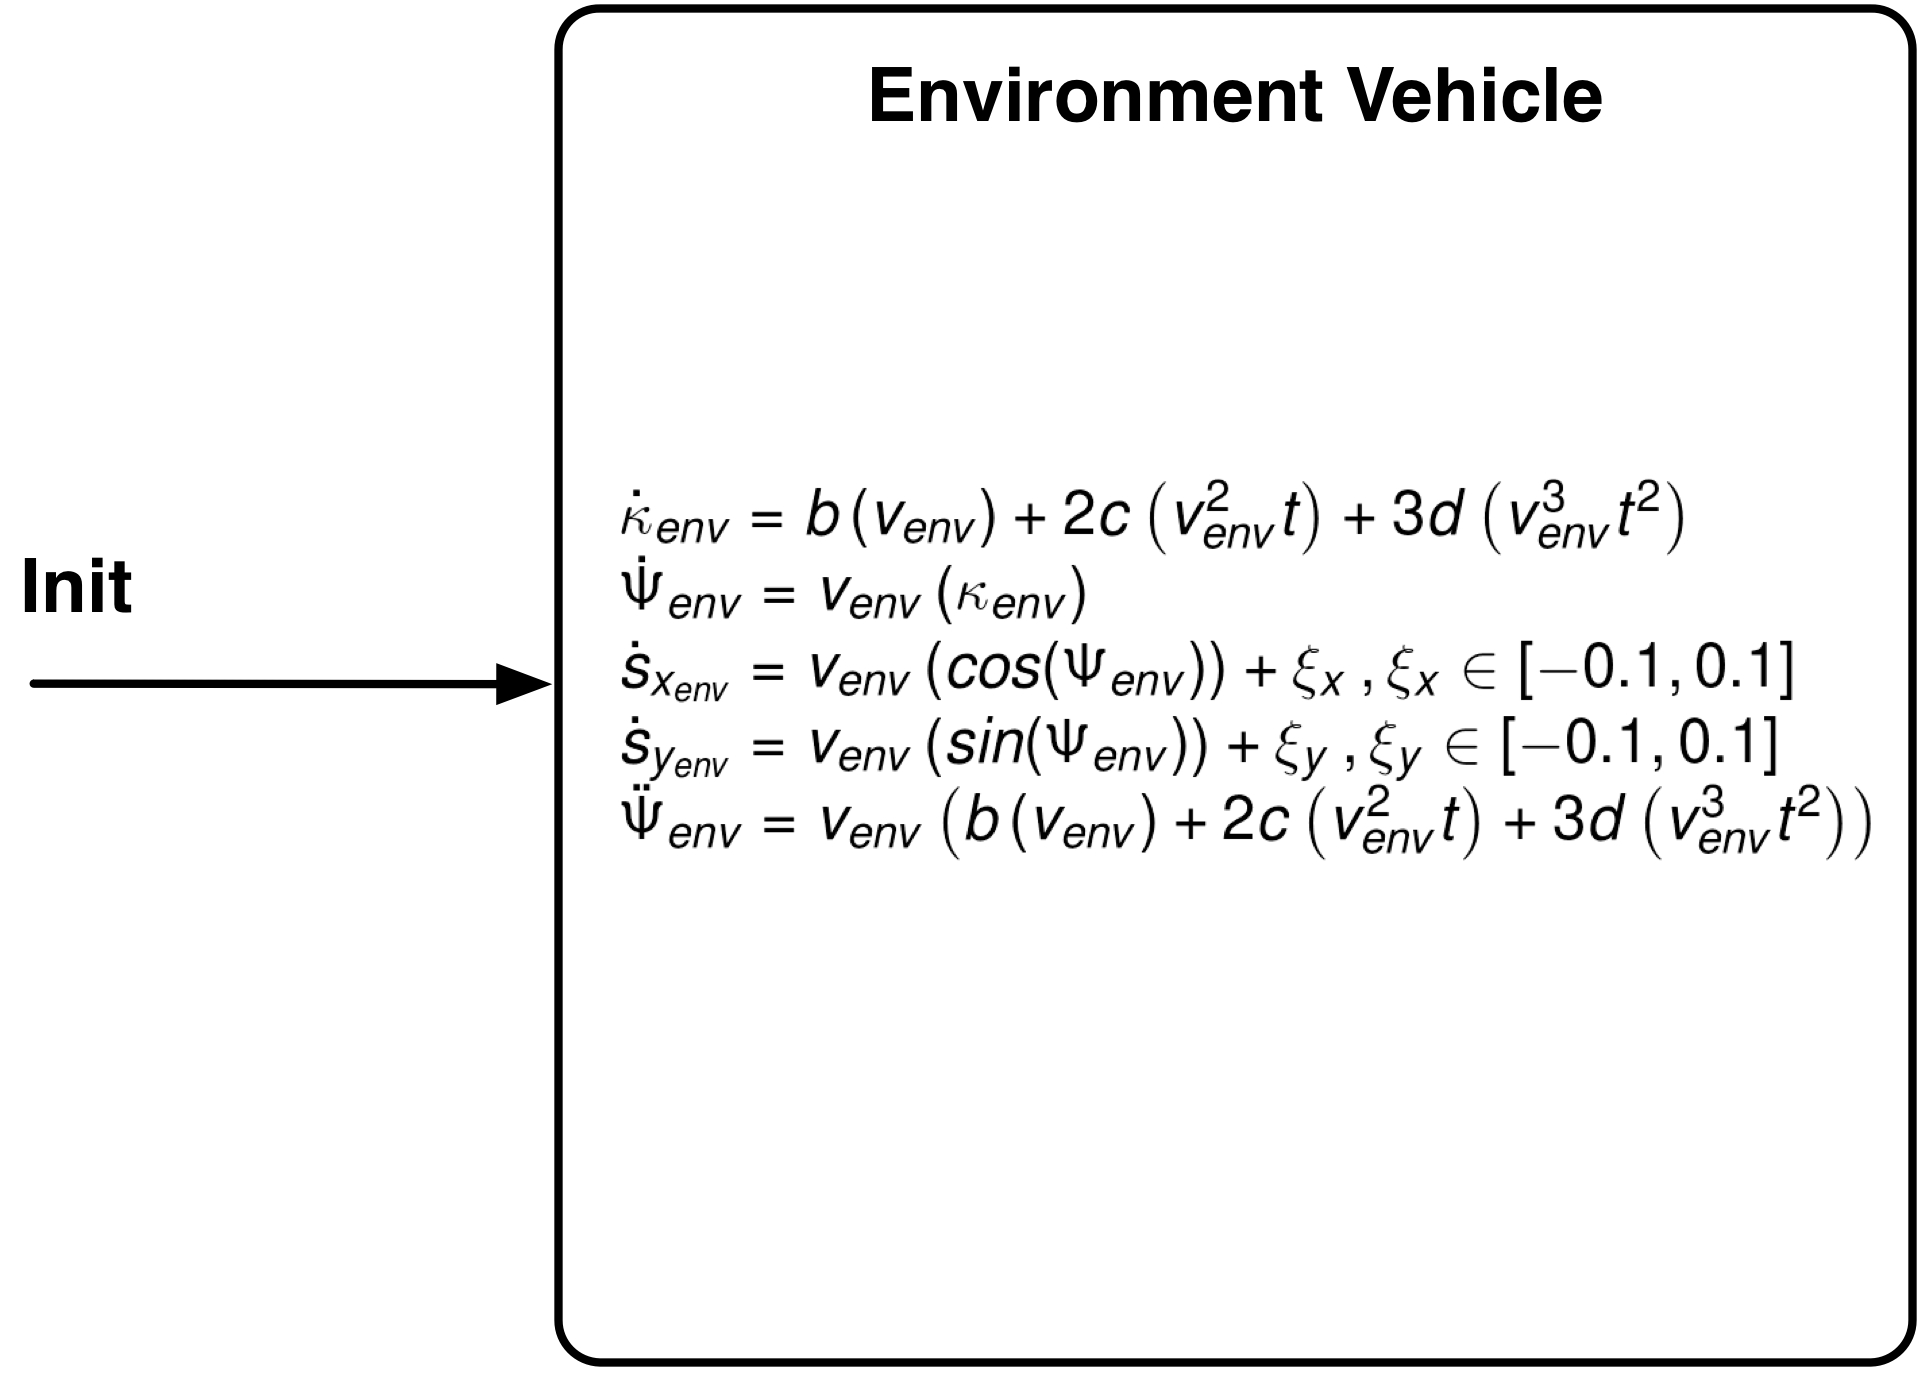
\includegraphics[scale=0.35]{figures/environment}
		\caption{Environment Vehicle Automaton}
	\end{figure}
		\begin{figure}[h]
			\centering
			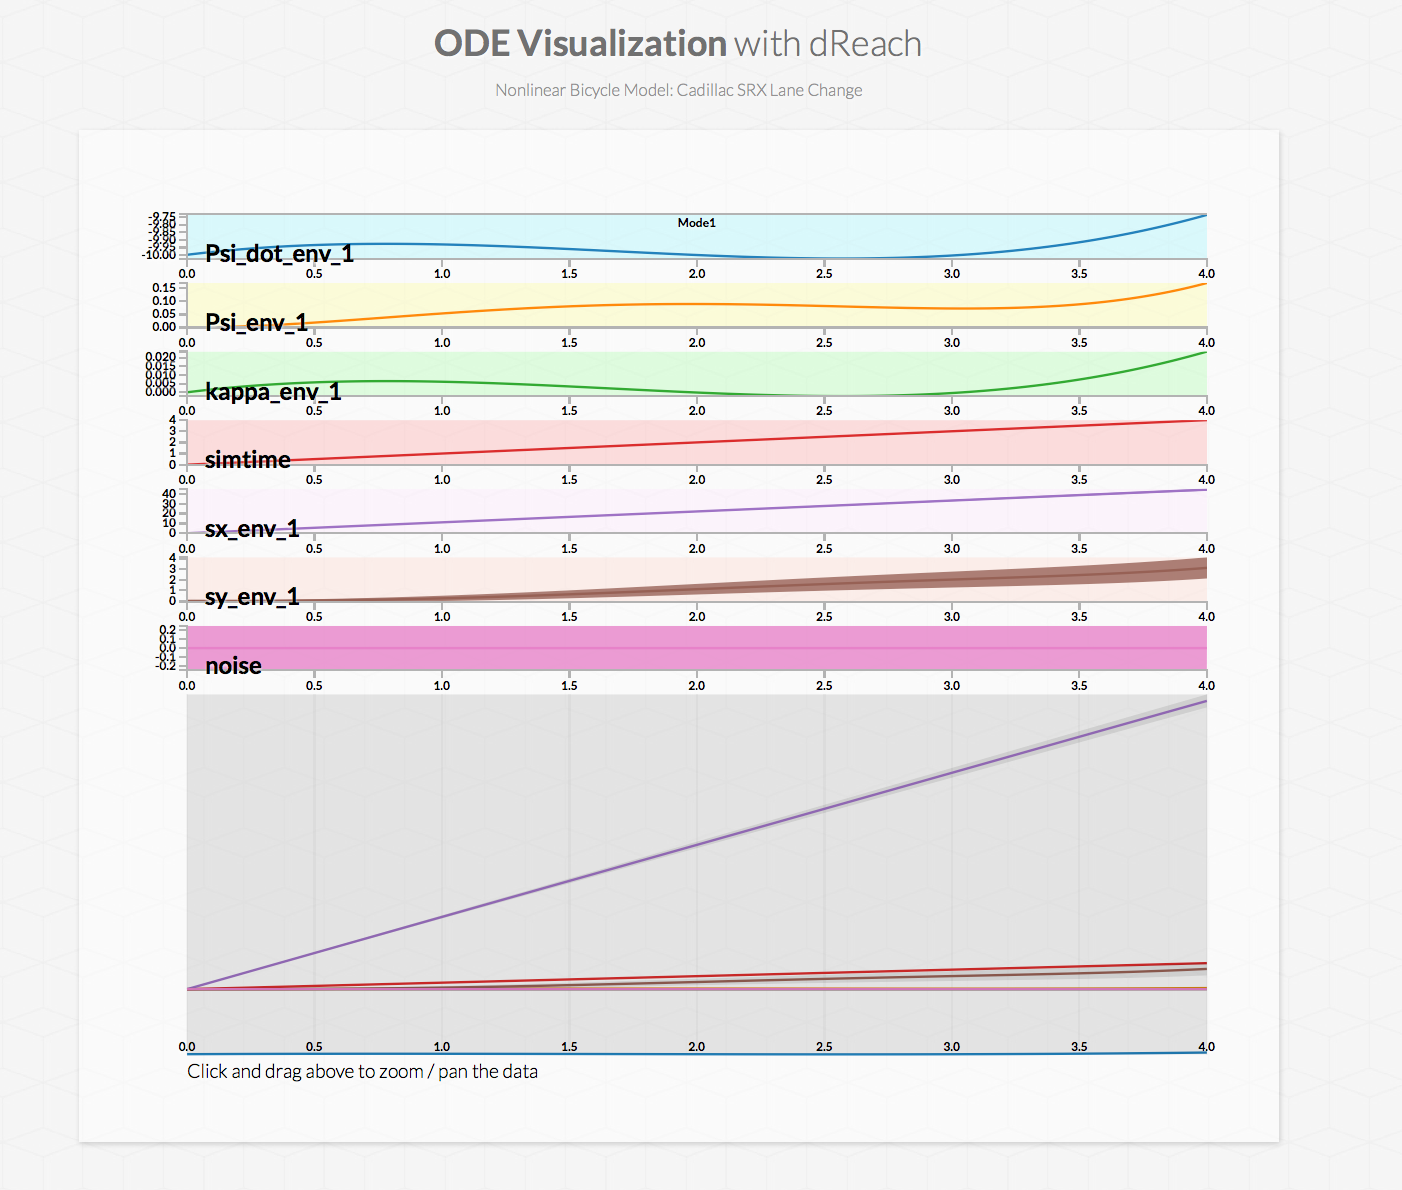
\includegraphics[width=\textwidth]{figures/dreachenv}
			\caption{Environment Vehicle Behavior Visualization}
		\end{figure}
The other vehicles operating within a scenario present both an interesting challenge and a primary motivation for formal verification. It is clear that it is impossible to know the intentions of the agents operating such vehicles; their execution represents a significant source of non-determinism. In fact, a more complex model of such agents which includes details such as steering angle or tire friction will not enable less conservative results, for it is the control input not the plant that remains the largest unknown. Thus, we conclude that:
{\it for verifying the autonomous agent, only the perceptible behavior of other agents is important, not their internal structure.}



Still it remains clear that {\it the behavior of other agents must be part of the scenario description.} As such we present a safety case which assumes that other agents will follow a certain minimal set of driving rules.

For brevity we will reference the following specification as $\xi$ in the case studies.% as specified in \cite{Althoff2014} which is a subset of the Vienna Convention on Road Traffic \cite{Europe.TransportDivision2007}: